%%%%%%%%%%%%%%%%%%%%%%%%%%%%%%%%%%%%%%%%%
% Lab Report Template
%
% Original author:
% Varun Singh (https://github.com/varunsingh29)
%
% Note:
%
%%%%%%%%%%%%%%%%%%%%%%%%%%%%%%%%%%%%%%%%%
\documentclass[a4paper,12pt]{article}

\author{Varun Singh}
\usepackage{fancyhdr} % Required for custom headers
%\usepackage{lastpage} % For X of XX style. Required to determine the last page for the footer
\usepackage{extramarks} % Required for headers and footers
\usepackage{graphicx} % Required to insert images
\usepackage{listings} % Required for insertion of code
\usepackage{lipsum} % Used for inserting dummy 'Lorem ipsum' text into the template


% Margins
\topmargin=-0.85in
\evensidemargin=0in
\oddsidemargin=-0.6cm
\textwidth=7.1in %Extra left margin for binding
\textheight=10.0in
\headsep=0.25in

\linespread{1.1} % Line spacing

% Set up the header and footer for first page
\fancypagestyle{firststyle}
{
\topmargin=-0.5in %Maintain header hieght for first page
\lhead{\Large Lab Exercise - 1} % Top left header
\chead{\firstxmark} %Top Center header
\rhead{\Large{\hmwkDueDate}}% Top right header
\lfoot{\hmwkAuthorName} % Bottom left footer
\cfoot{\lastxmark} % Bottom center footer
\rfoot{Page\ \thepage}
\setcounter{page}{1} % For Custom Page numbers
%\rfoot{Page\ \thepage\ of \pageref{LastPage}} % Bottom right footer
\renewcommand\headrulewidth{0.4pt} % Size of the header rule
\renewcommand\footrulewidth{0.4pt} % Size of the footer rule
}

% Set up the header and footer for other pages
\pagestyle{fancy}
\lfoot{\hmwkAuthorName} % Bottom left footer
\cfoot{\lastxmark} % Bottom center footer
\rfoot{Page\ \thepage}
%\rfoot{Page\ \thepage\ of \pageref{LastPage}} % Bottom right footer
\renewcommand\headrulewidth{0pt} % Size of the header rule
\renewcommand\footrulewidth{0.4pt} % Size of the footer rule

\setlength\parindent{0pt} % Removes all indentation from paragraphs

%----------------------------------------------------------------------------------------
%	NAME AND CLASS SECTION
%----------------------------------------------------------------------------------------

\newcommand{\hmwkTitle}{Assignment\ \#1} % Assignment title
\newcommand{\hmwkAuthorName}{Varun Singh - 141357} % Your name
\newcommand{\hmwkDueDate}{Monday,\ July\ 17,\ 2016} % Due date

%---------------------------------


\begin{document}

\thispagestyle{firststyle}
\textbf{Ques 1: }
\begin{minipage}[t]{16cm}
\lipsum[1]
%\begin{itemize} %For bulleted lists
%\itemsep-0.5em
%\item Check for this shit
%\item Check for that shit
%\end{itemize}
\end{minipage}\\ \\
\textbf{Solution:}
\begin{minipage}[t]{16cm}
\lipsum[2]
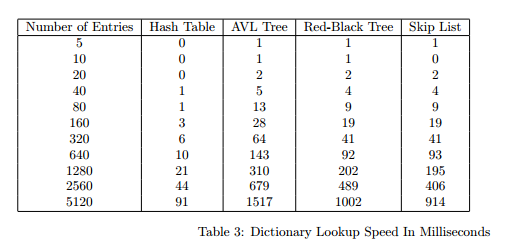
\includegraphics{1.PNG}\\
\lipsum[1] Adding more text jkfshfkjsdhfsjhflsjhfsfsfhslfjshfshhfsjfsfhskjfhskjfhsjfss
sfkjshfksjhfkj sldfj lskgdjlskg lsdjgslkdgjsgk sj;gljs;gs;g
sgdlgjhslgjshglshgslghslghslghsldkhlkh lfshslgshldgshlgshdglsghslghslghslghsldgskgslgslhlldkhlhslfhslkfhslkdfhslkfshlfshfslfk
slkdhfslhfslfhslfksflsfhslkfhslkfhslkhlshlkkjhkj
slhdfsjdhflsjfhlshflshflsfsf
\end{minipage}

\newpage
\begin{flushright}
\begin{minipage}[tx]{16.1cm} %For continued text
Hello people \lipsum[5]
\end{minipage}\\
\end{flushright}

%\rule{\linewidth}{1pt} \\ % To insert horizontal divider
\textbf{Ques 2: }
\begin{minipage}[t]{16cm}
\lipsum[1]
%\begin{itemize} %For bulleted lists
%\itemsep-0.5em
%\item Check for this shit
%\item Check for that shit
%\end{itemize}
\end{minipage}\\ \\
\textbf{Solution:}
\begin{minipage}[t]{16cm}
\lipsum[2]
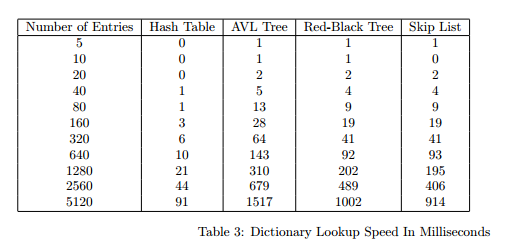
\includegraphics{1.PNG}
\end{minipage}
\end{document}
